\section{自己紹介}
こんにちは、あわあわくん()(@materialofmouse)です。
同人誌を書く話になったのでLEDでひたすら発電してみました。
この章ではLEDで発電という普通はやらないことをやっています。
それに検証性がないのでちゃんと書かれてません。おまけだとおもって読んでください。

\section{実際に発電してみる}
LEDで発電できるのか、実際に試したいと思います。
ものが用意できる方はぜひやってみてください。

\begin{description}
  \item[場所]{近くの駐車場}
  \item[時間]{14:10}
  \item[光源]{太陽光}
  \item[照度]{$160,000\si\lux$}
  \item[天気]{雲ひとつない晴れ}
\end{description}


\subsection{LED1個}
まず、LEDを1個。アノード側にテスターのプラス、カソード側にテスターのマイナスを接続します。
図\ref{fig:led1}の状態でLEDを太陽の方へ向けてみます。そこで発生した電流と電圧の値を取っていきます。
手元の環境では、普通の白色LEDから約10$\mu\si\ampere$,約1.2$\si\volt$発生しました。

\begin{figure}[htbp]
    \centering
    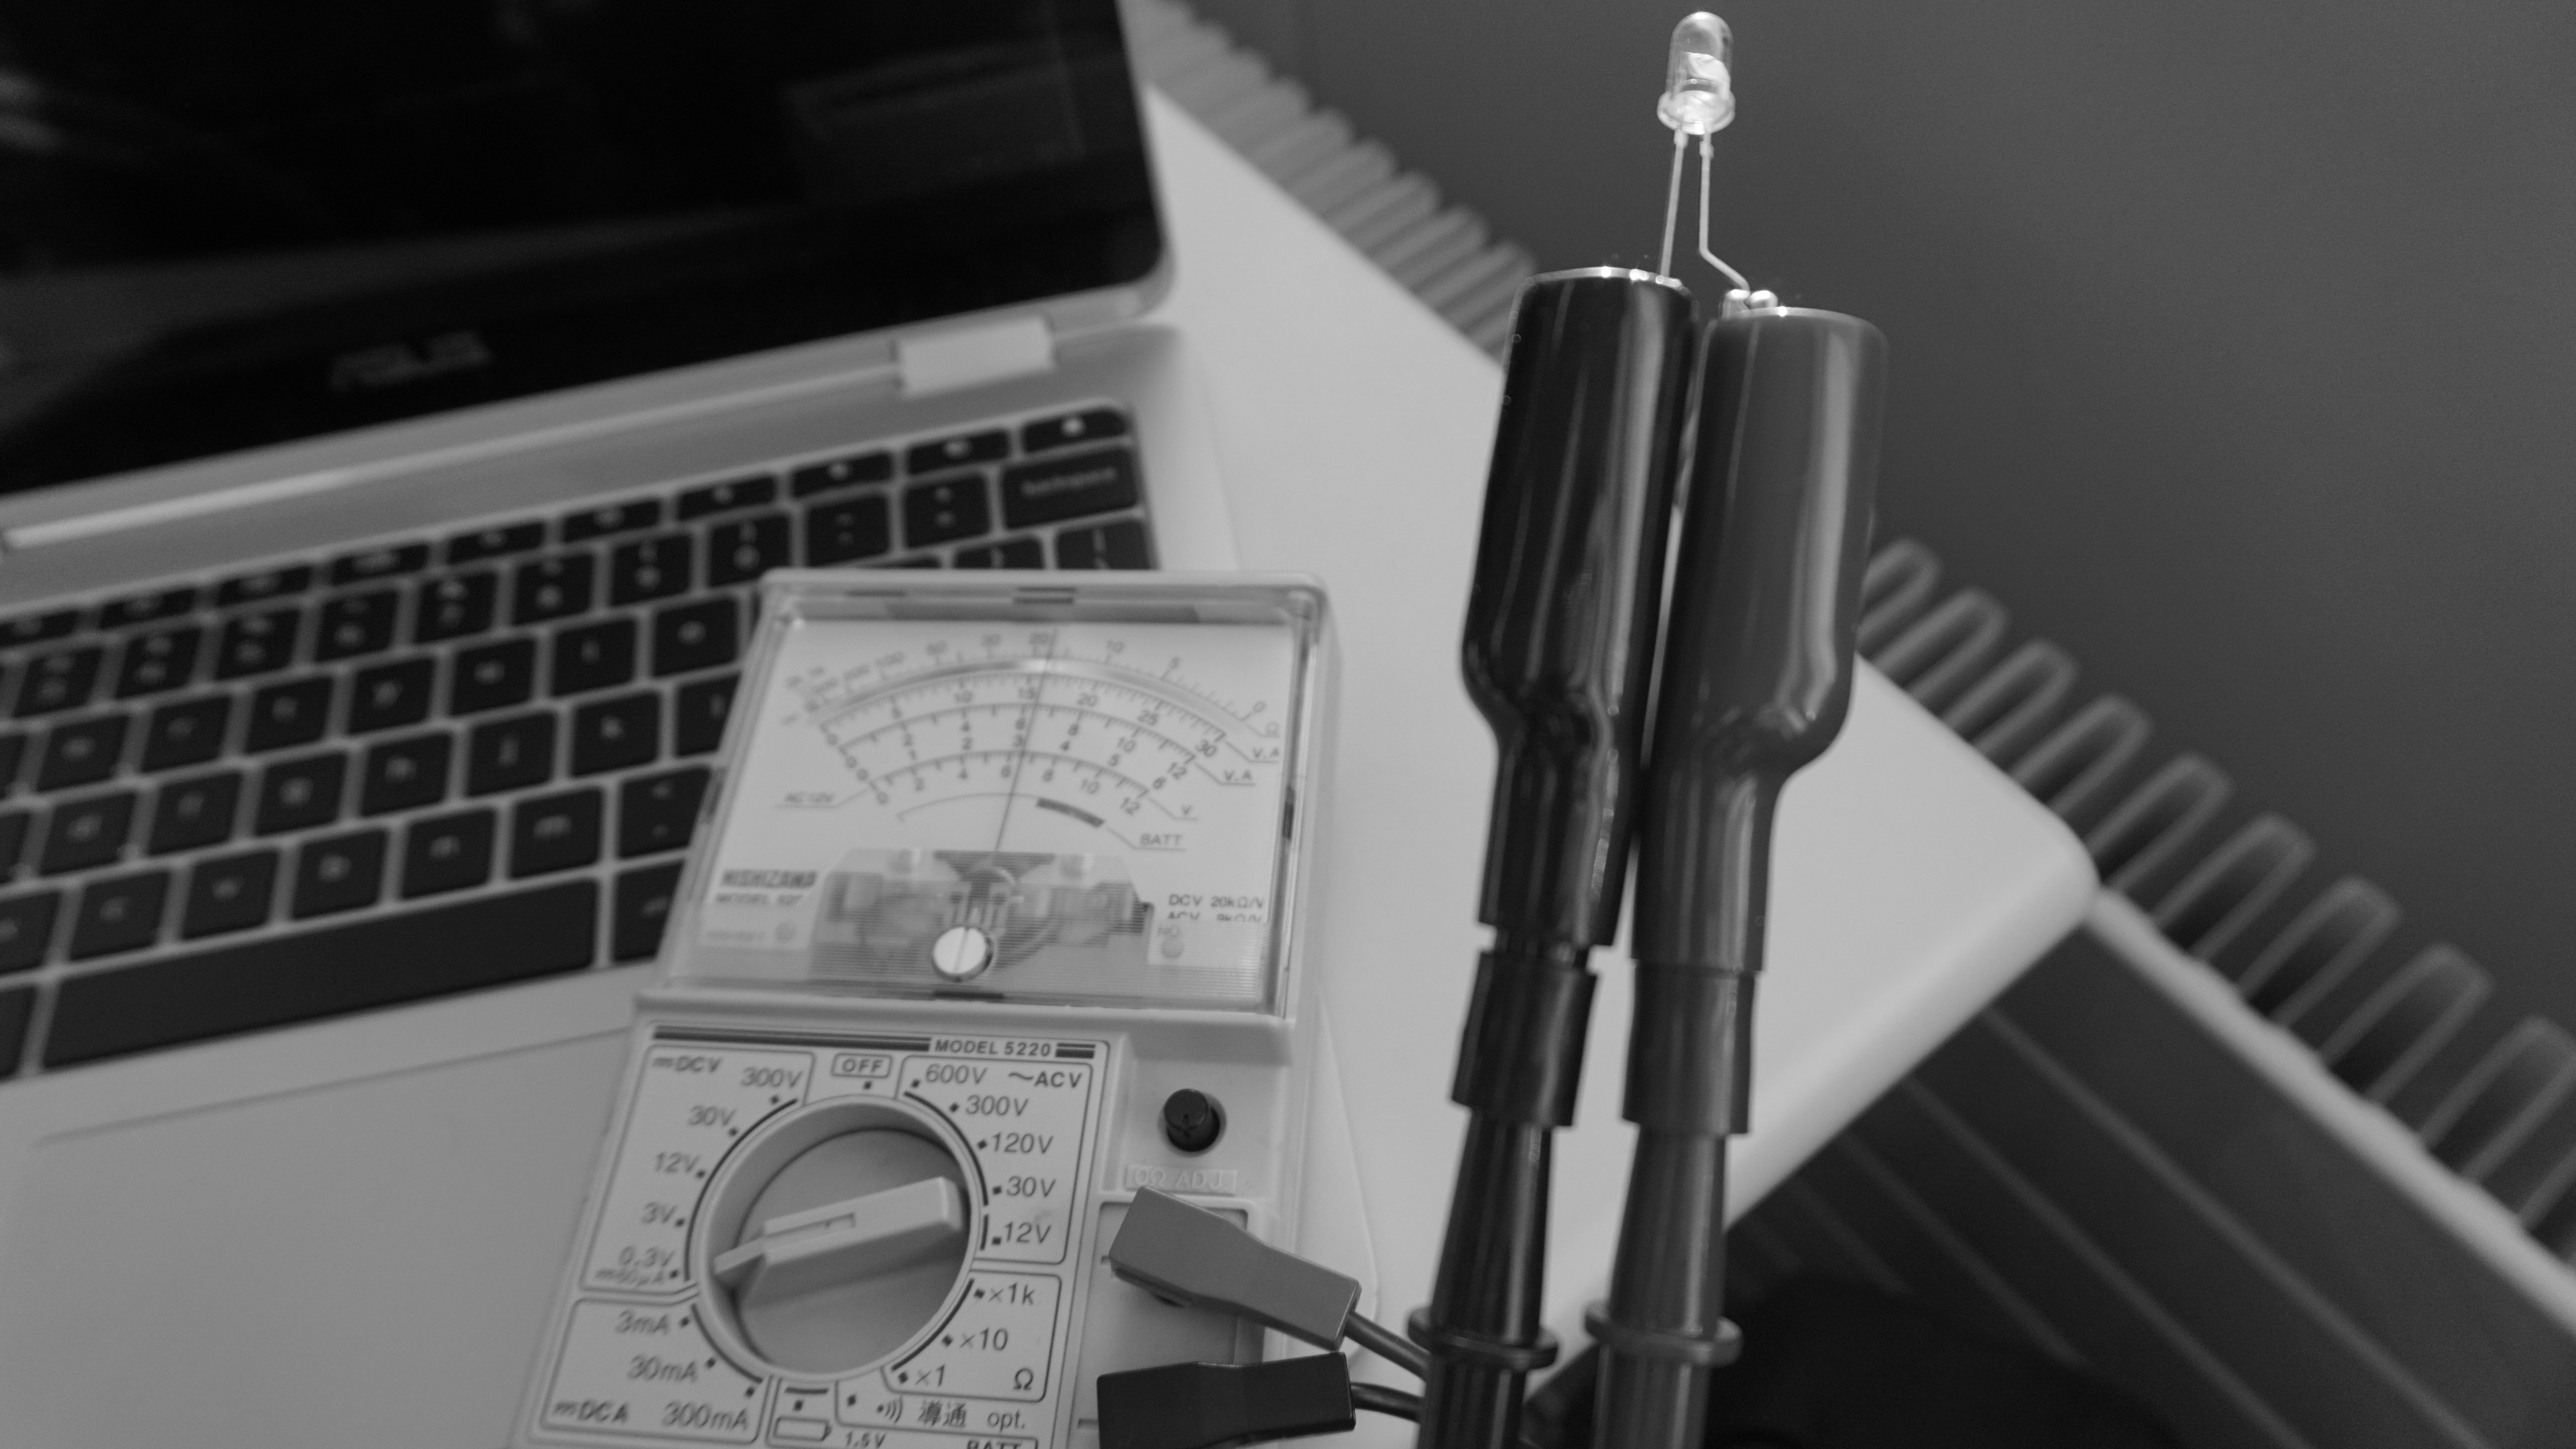
\includegraphics[width=60mm]{./assets/mouse/gray/1.JPG}
    \caption{LED1個で電流と電圧を測定している様子}
    \label{fig:led1}
\end{figure}

\subsection{直列と並列どちらが良いのか考える}
複数接続するにあたり、直列接続と並列接続のどちらが発電に適しているのかを実験してみました。

LED2個を直列に接続し、その両端をテスターで見ていきます。
図\ref{fig:led2}に測定の様子を示します.
そこに光を与えたところ、約100$\mu\si\ampere$,約2.5$\si\volt$発生しました。
この結果から、LED1個の時と比べ、電流、電圧ともに2倍になっていることがわかります。

\begin{figure}[htbp]
    \centering
    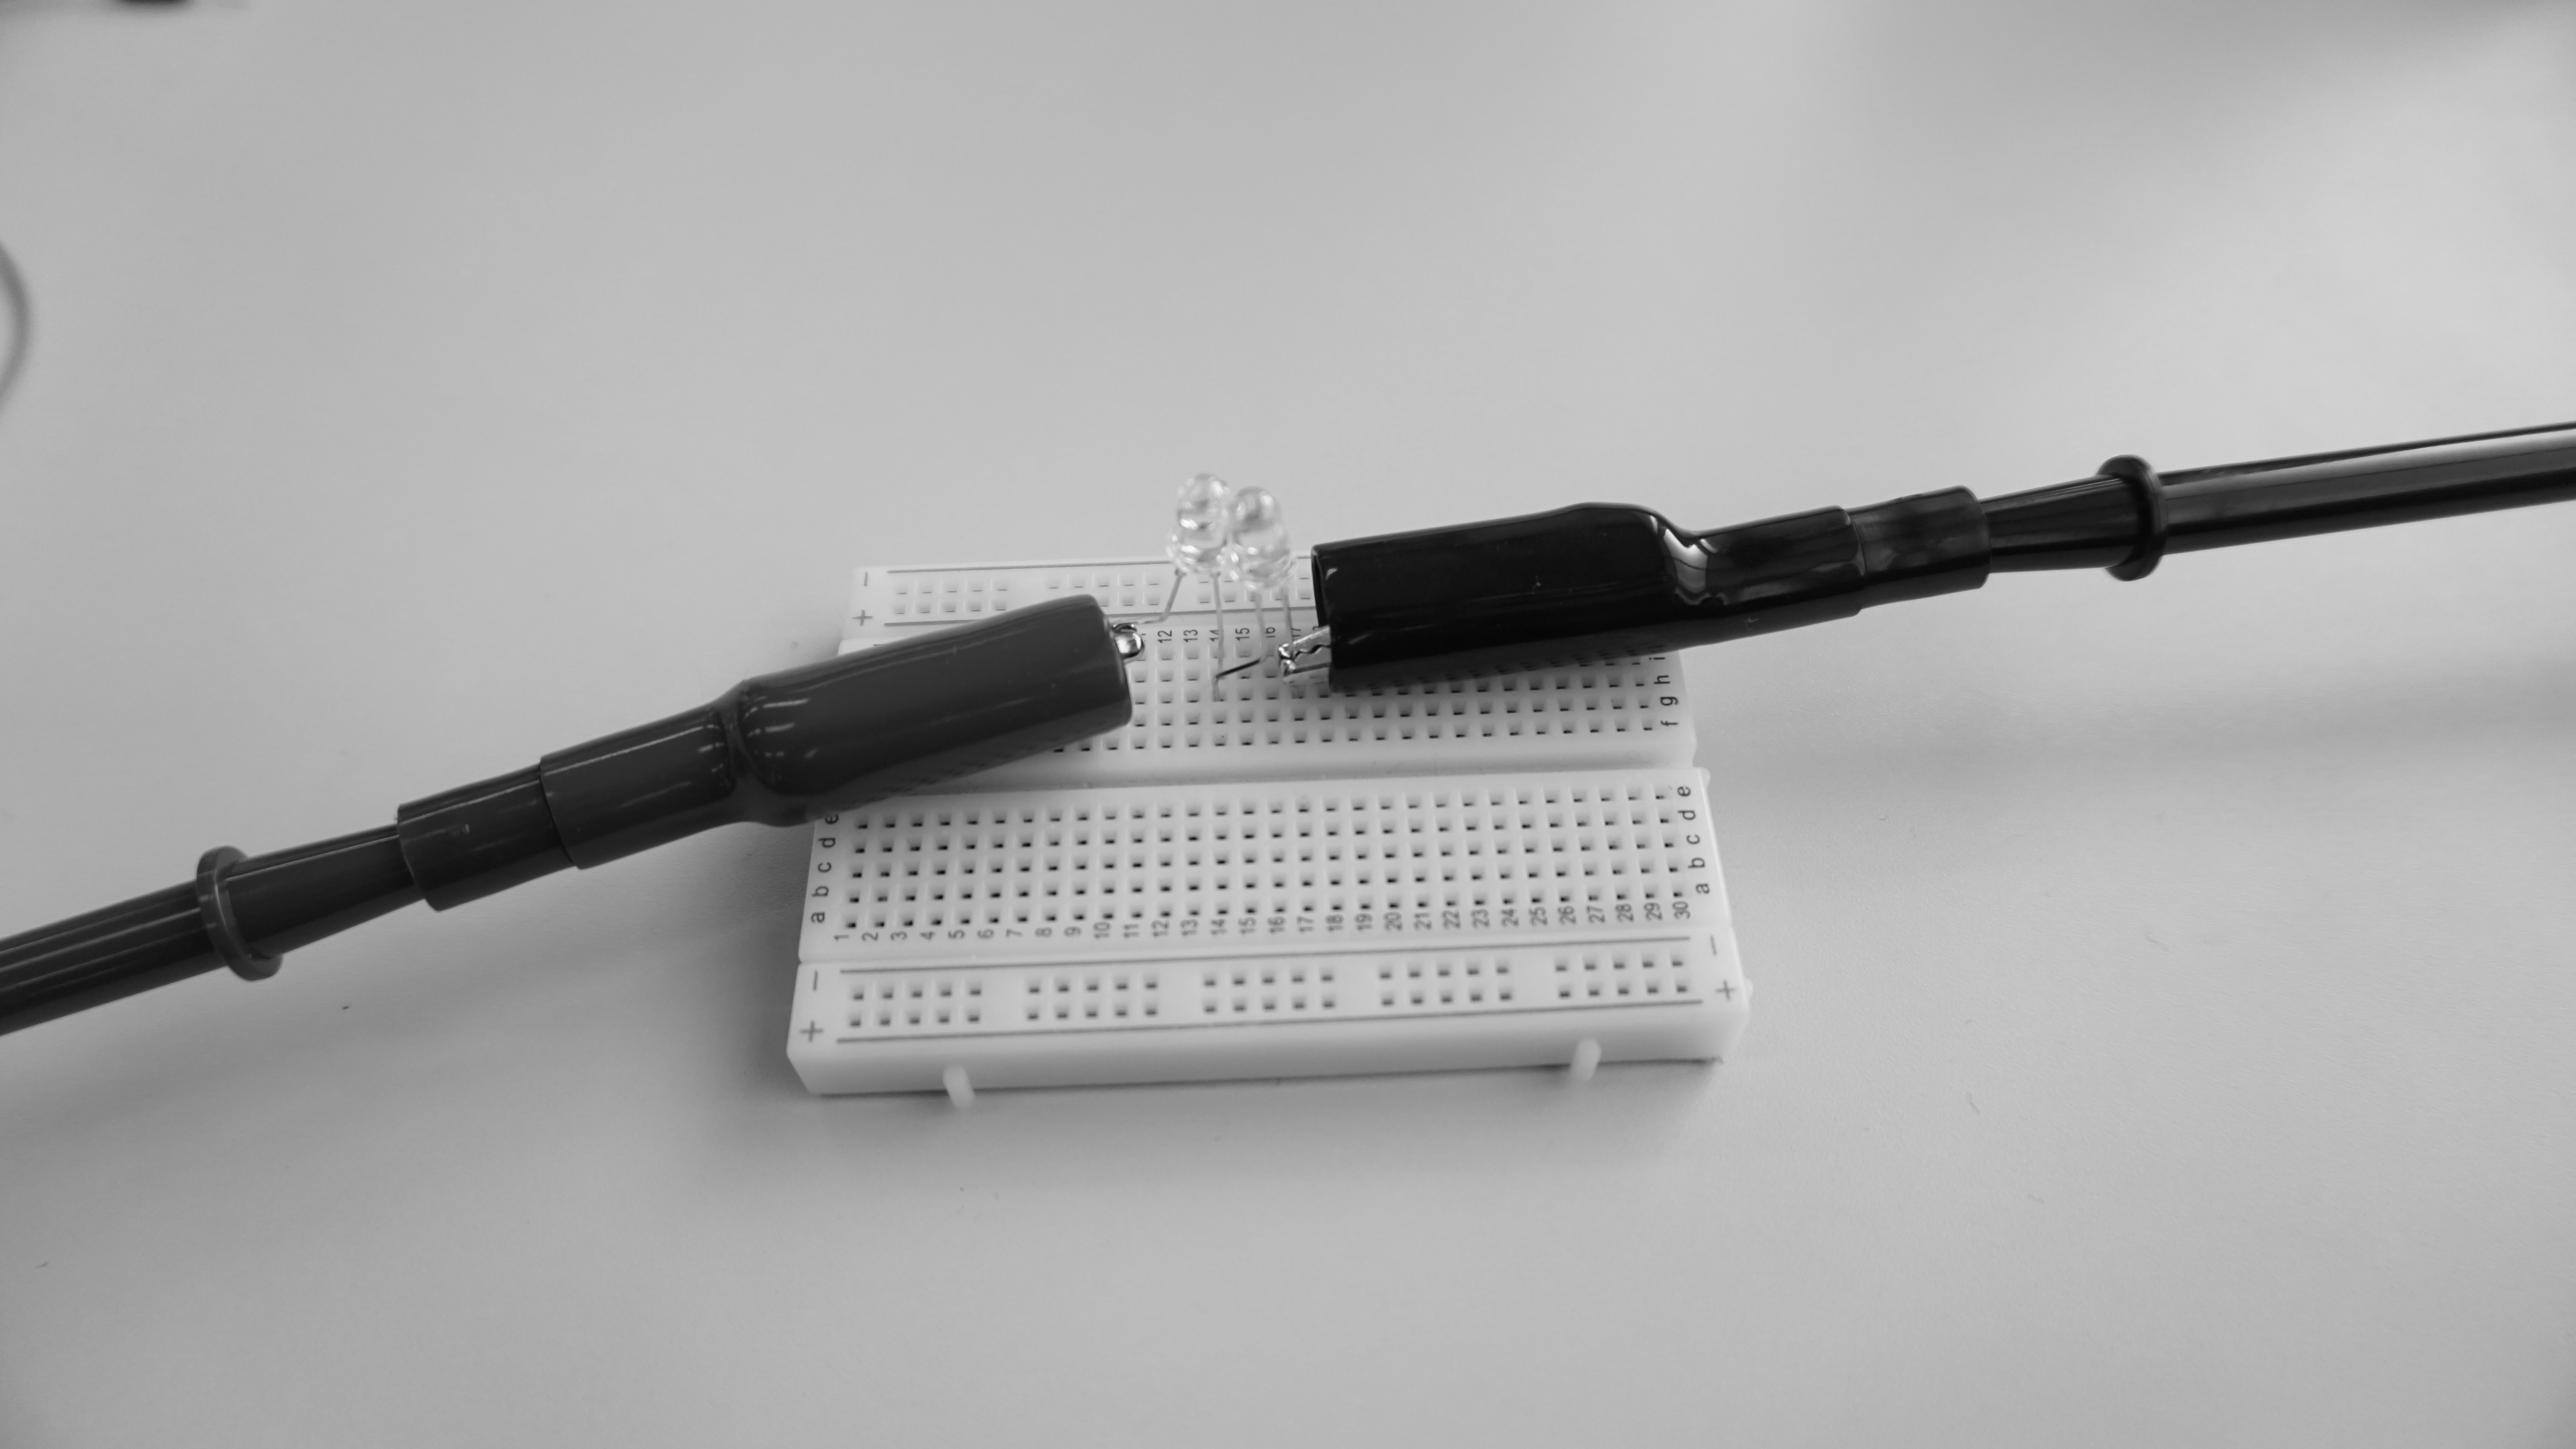
\includegraphics[width=60mm]{./assets/mouse/gray/12.JPG}
    \caption{LED2個で電流と電圧を測定している様子}
    \label{fig:led2}
\end{figure}

次に図\ref{fig:led10}のようにLED10個を直列に接続し、同じくその両端をテスターで見てみました。
その結果、約110$\mu\si\ampere$,約0.5$\si\volt$発生しました。
LED2個の時と比べて電圧が極端に小さくなっていることがわかります。
これはおそらく、LEDの電圧降下の影響をもろに受けてしまったためだと思います。
電流値は、なんかいい感じです。
結果としては、{\bf 並列接続のほうがいい}


\begin{figure}[htbp]
    \centering
    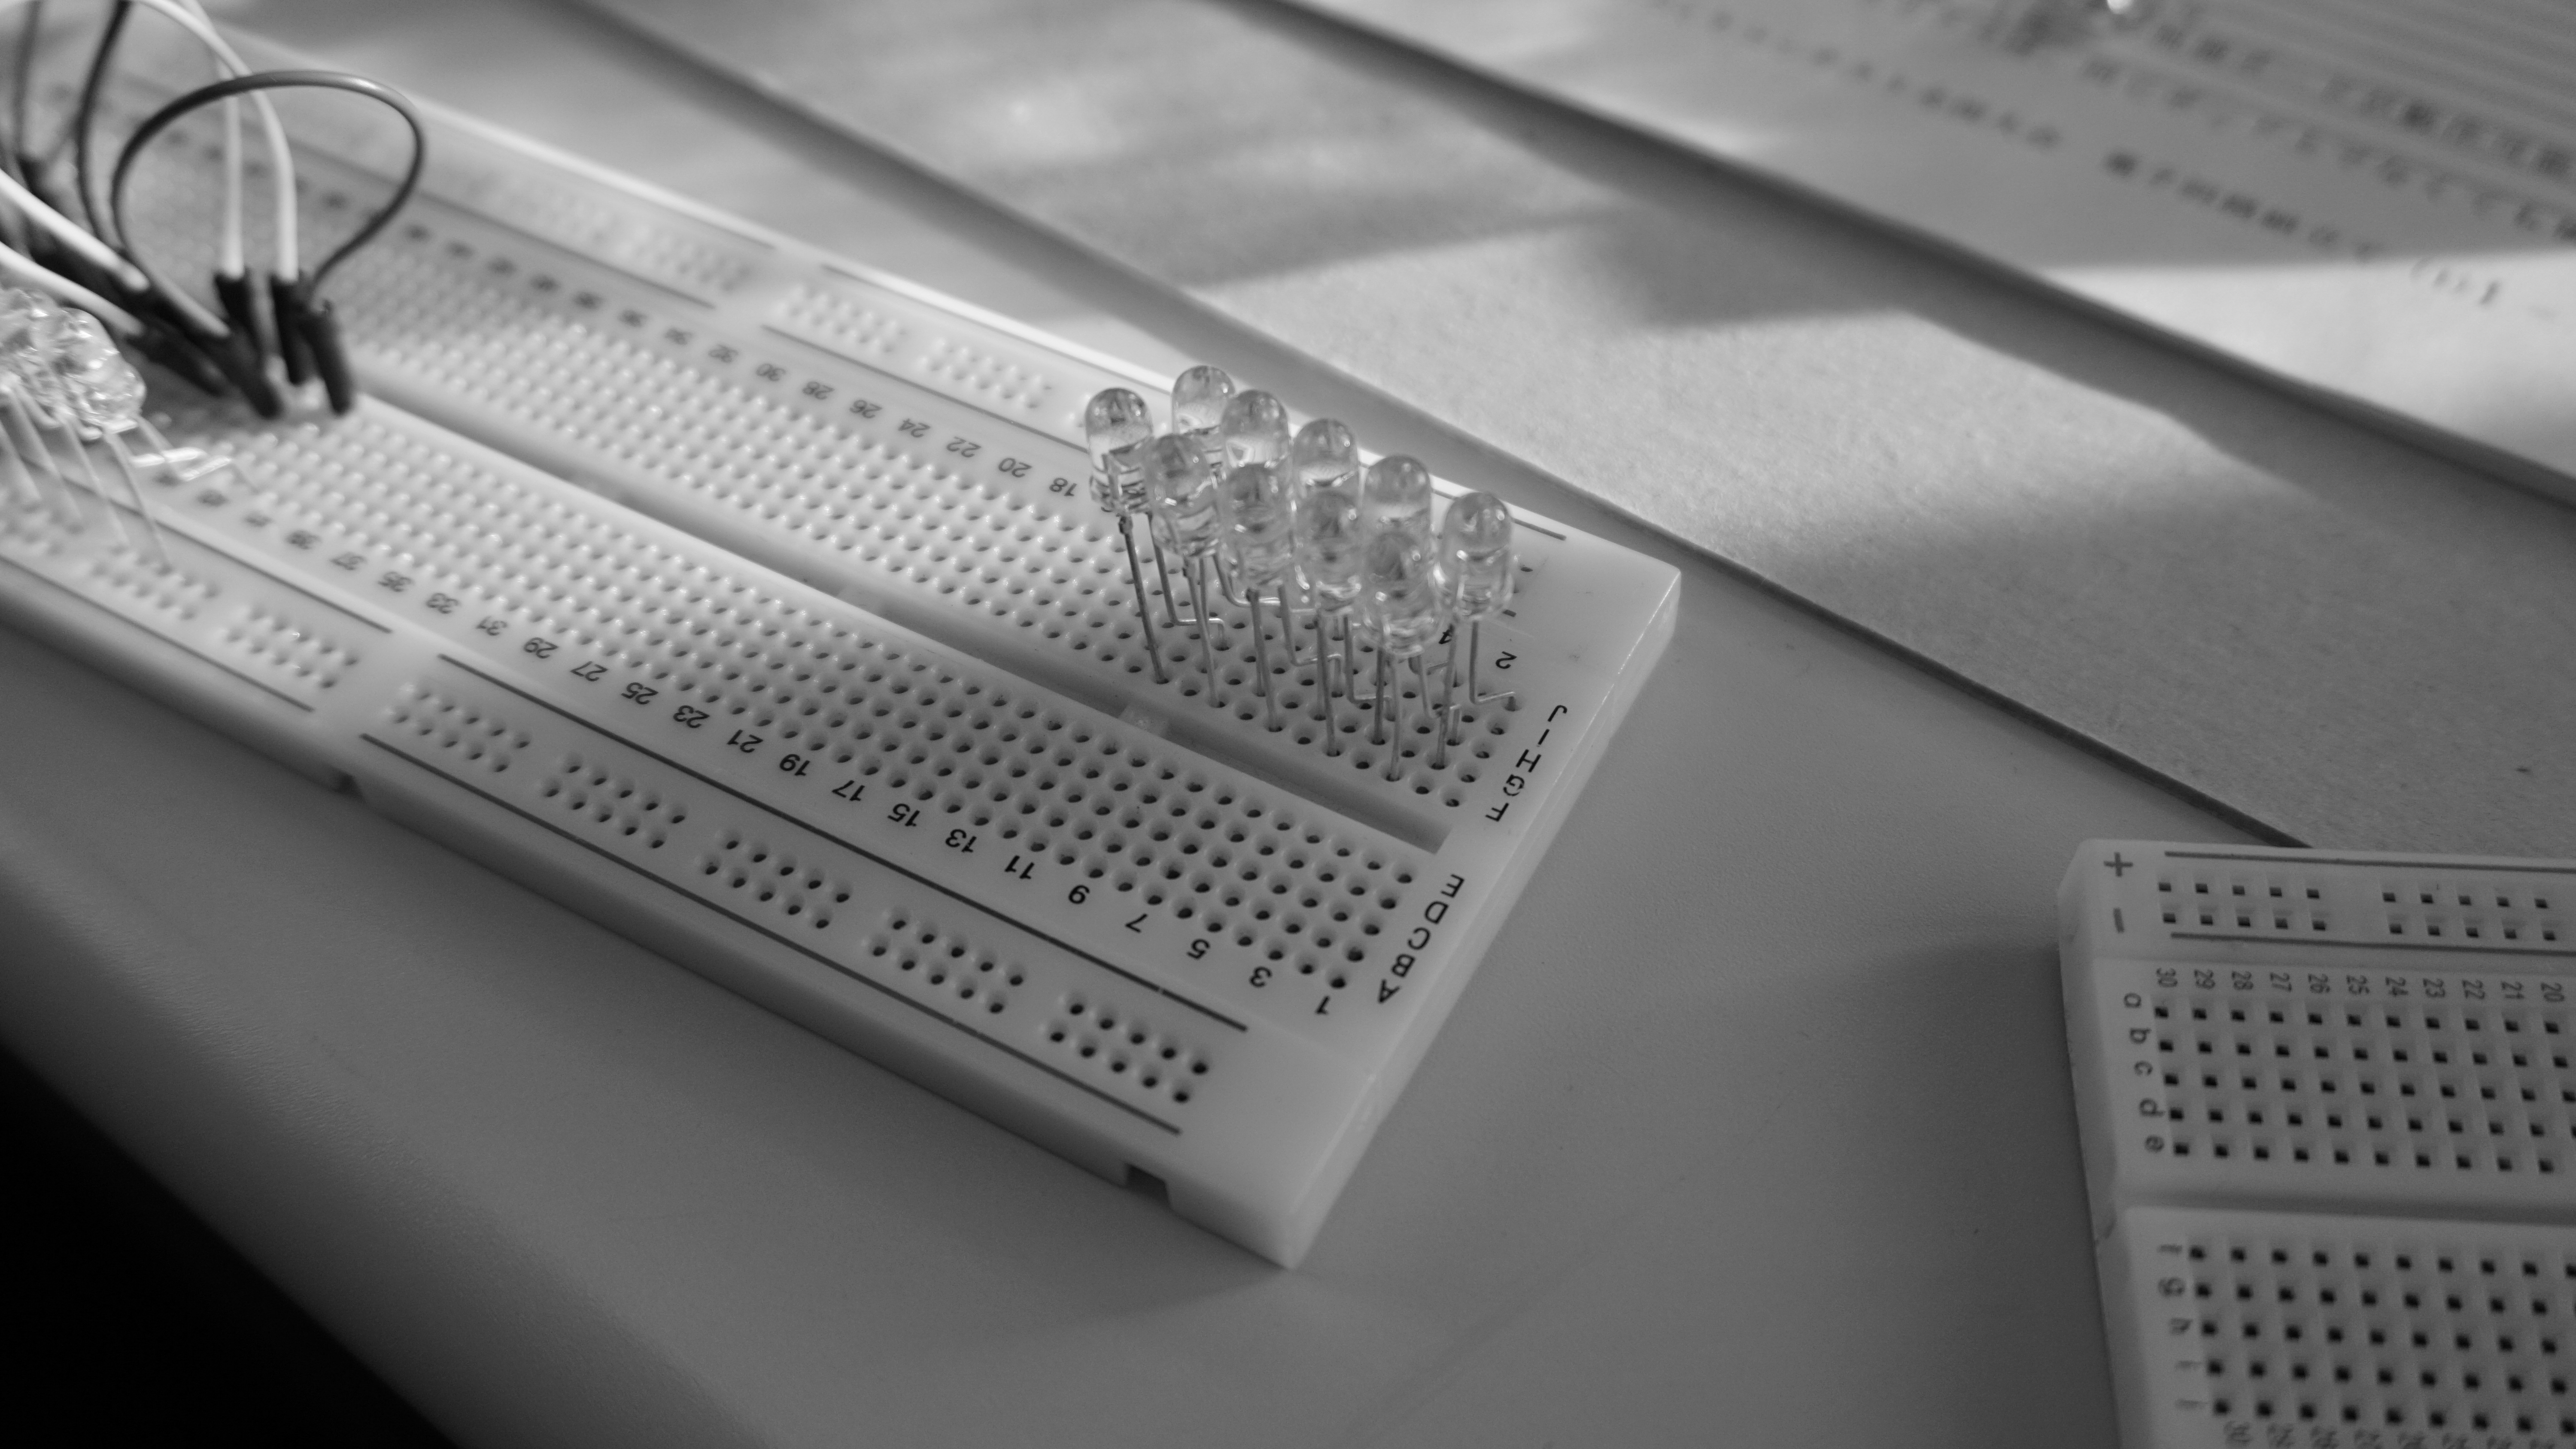
\includegraphics[width=60mm]{./assets/mouse/gray/4.JPG}
    \caption{10個のLEDを接続しているブレッドボード}
    \label{fig:led10}
\end{figure}

図\ref{fig:led_par}のようにLED2個を並列に接続し、同じくテスターで見ていきます。
こちらも太陽光で、同じ時間帯に実験しました。
並列接続の場合、約100$\mu\si\ampere$,1.5$\si\volt$発生しました。


\begin{figure}[htbp]
    \centering
    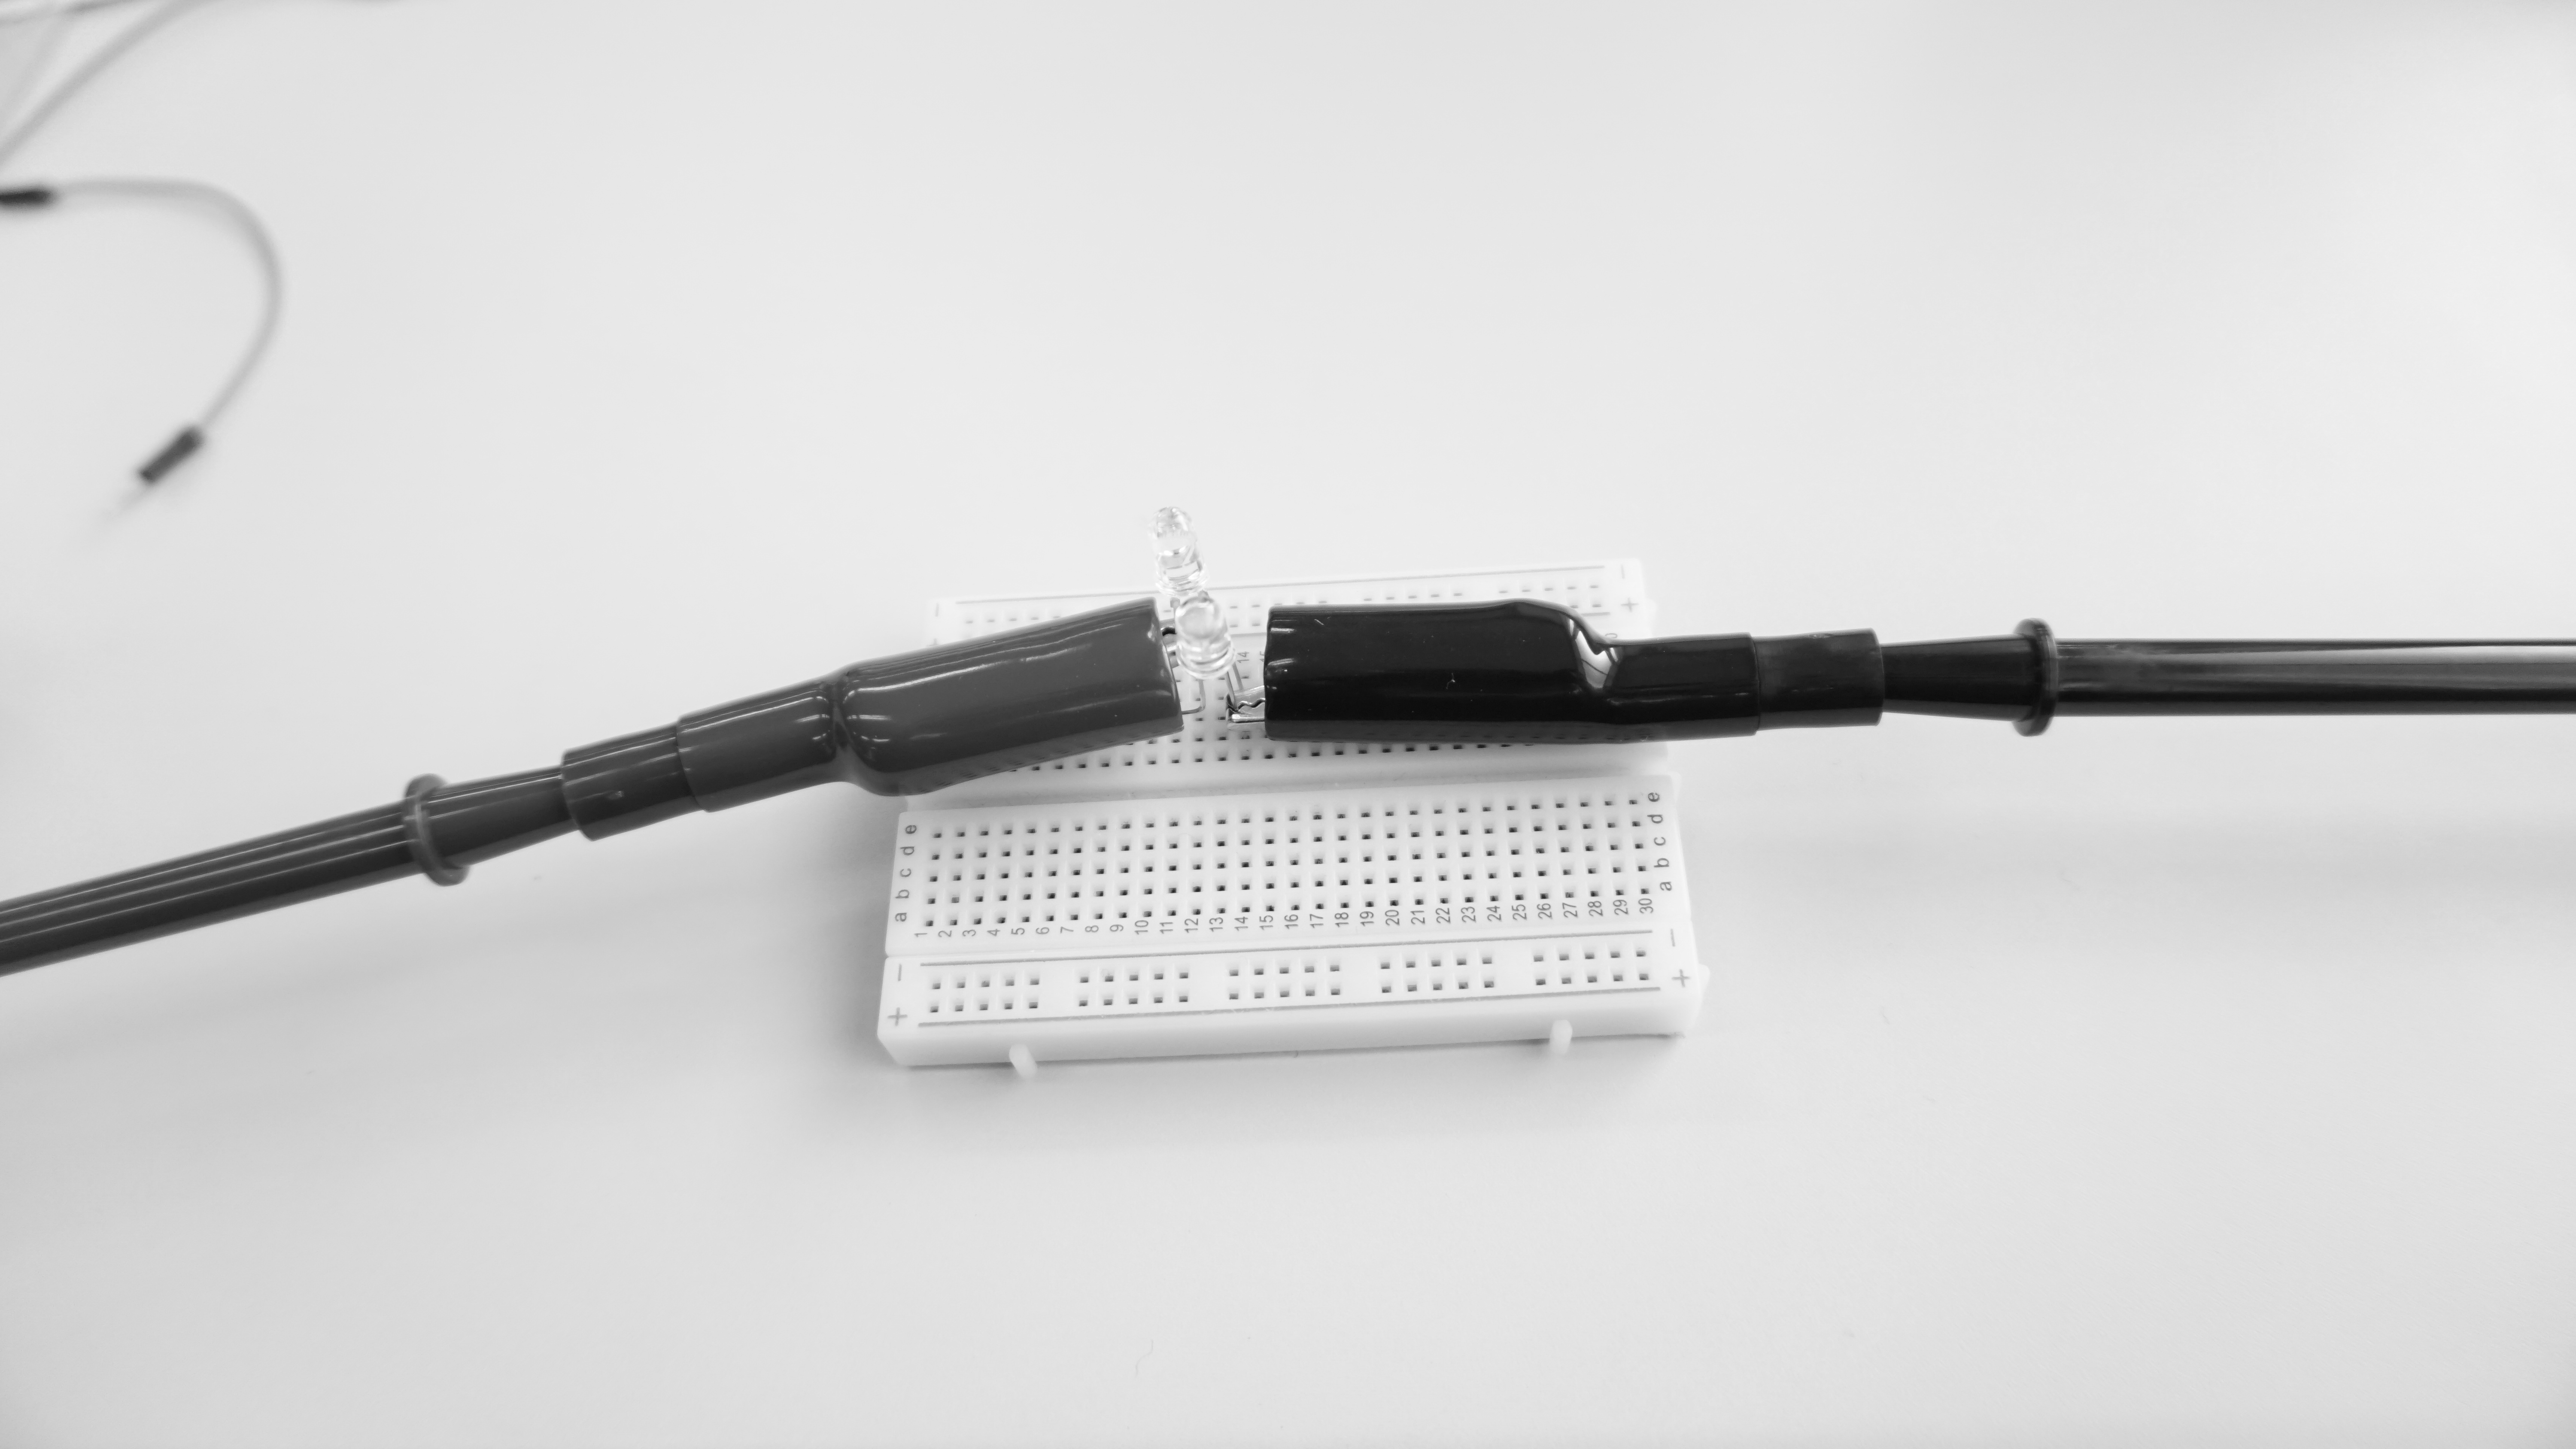
\includegraphics[width=60mm]{./assets/mouse/gray/13.JPG}
    \caption{並列接続したLEDの電流と電圧を測定している様子}
    \label{fig:led_par}
\end{figure}


先ほどと同じく、図\ref{fig:led_par10}のようにLED10個を並列に並べたものの値を取っていきます。
こちらも同じく太陽光で、同じ時間帯です。
この環境で約0.4\si{\milli\ampere},1.5$\si\volt$発生しました。やっと現実味のある数値になってきました。
これは直列と違い抵抗が並列に接続されているためだと思われます。
よくわからないけどいきなり電流が大きくなりました。


\begin{figure}[htbp]
    \centering
    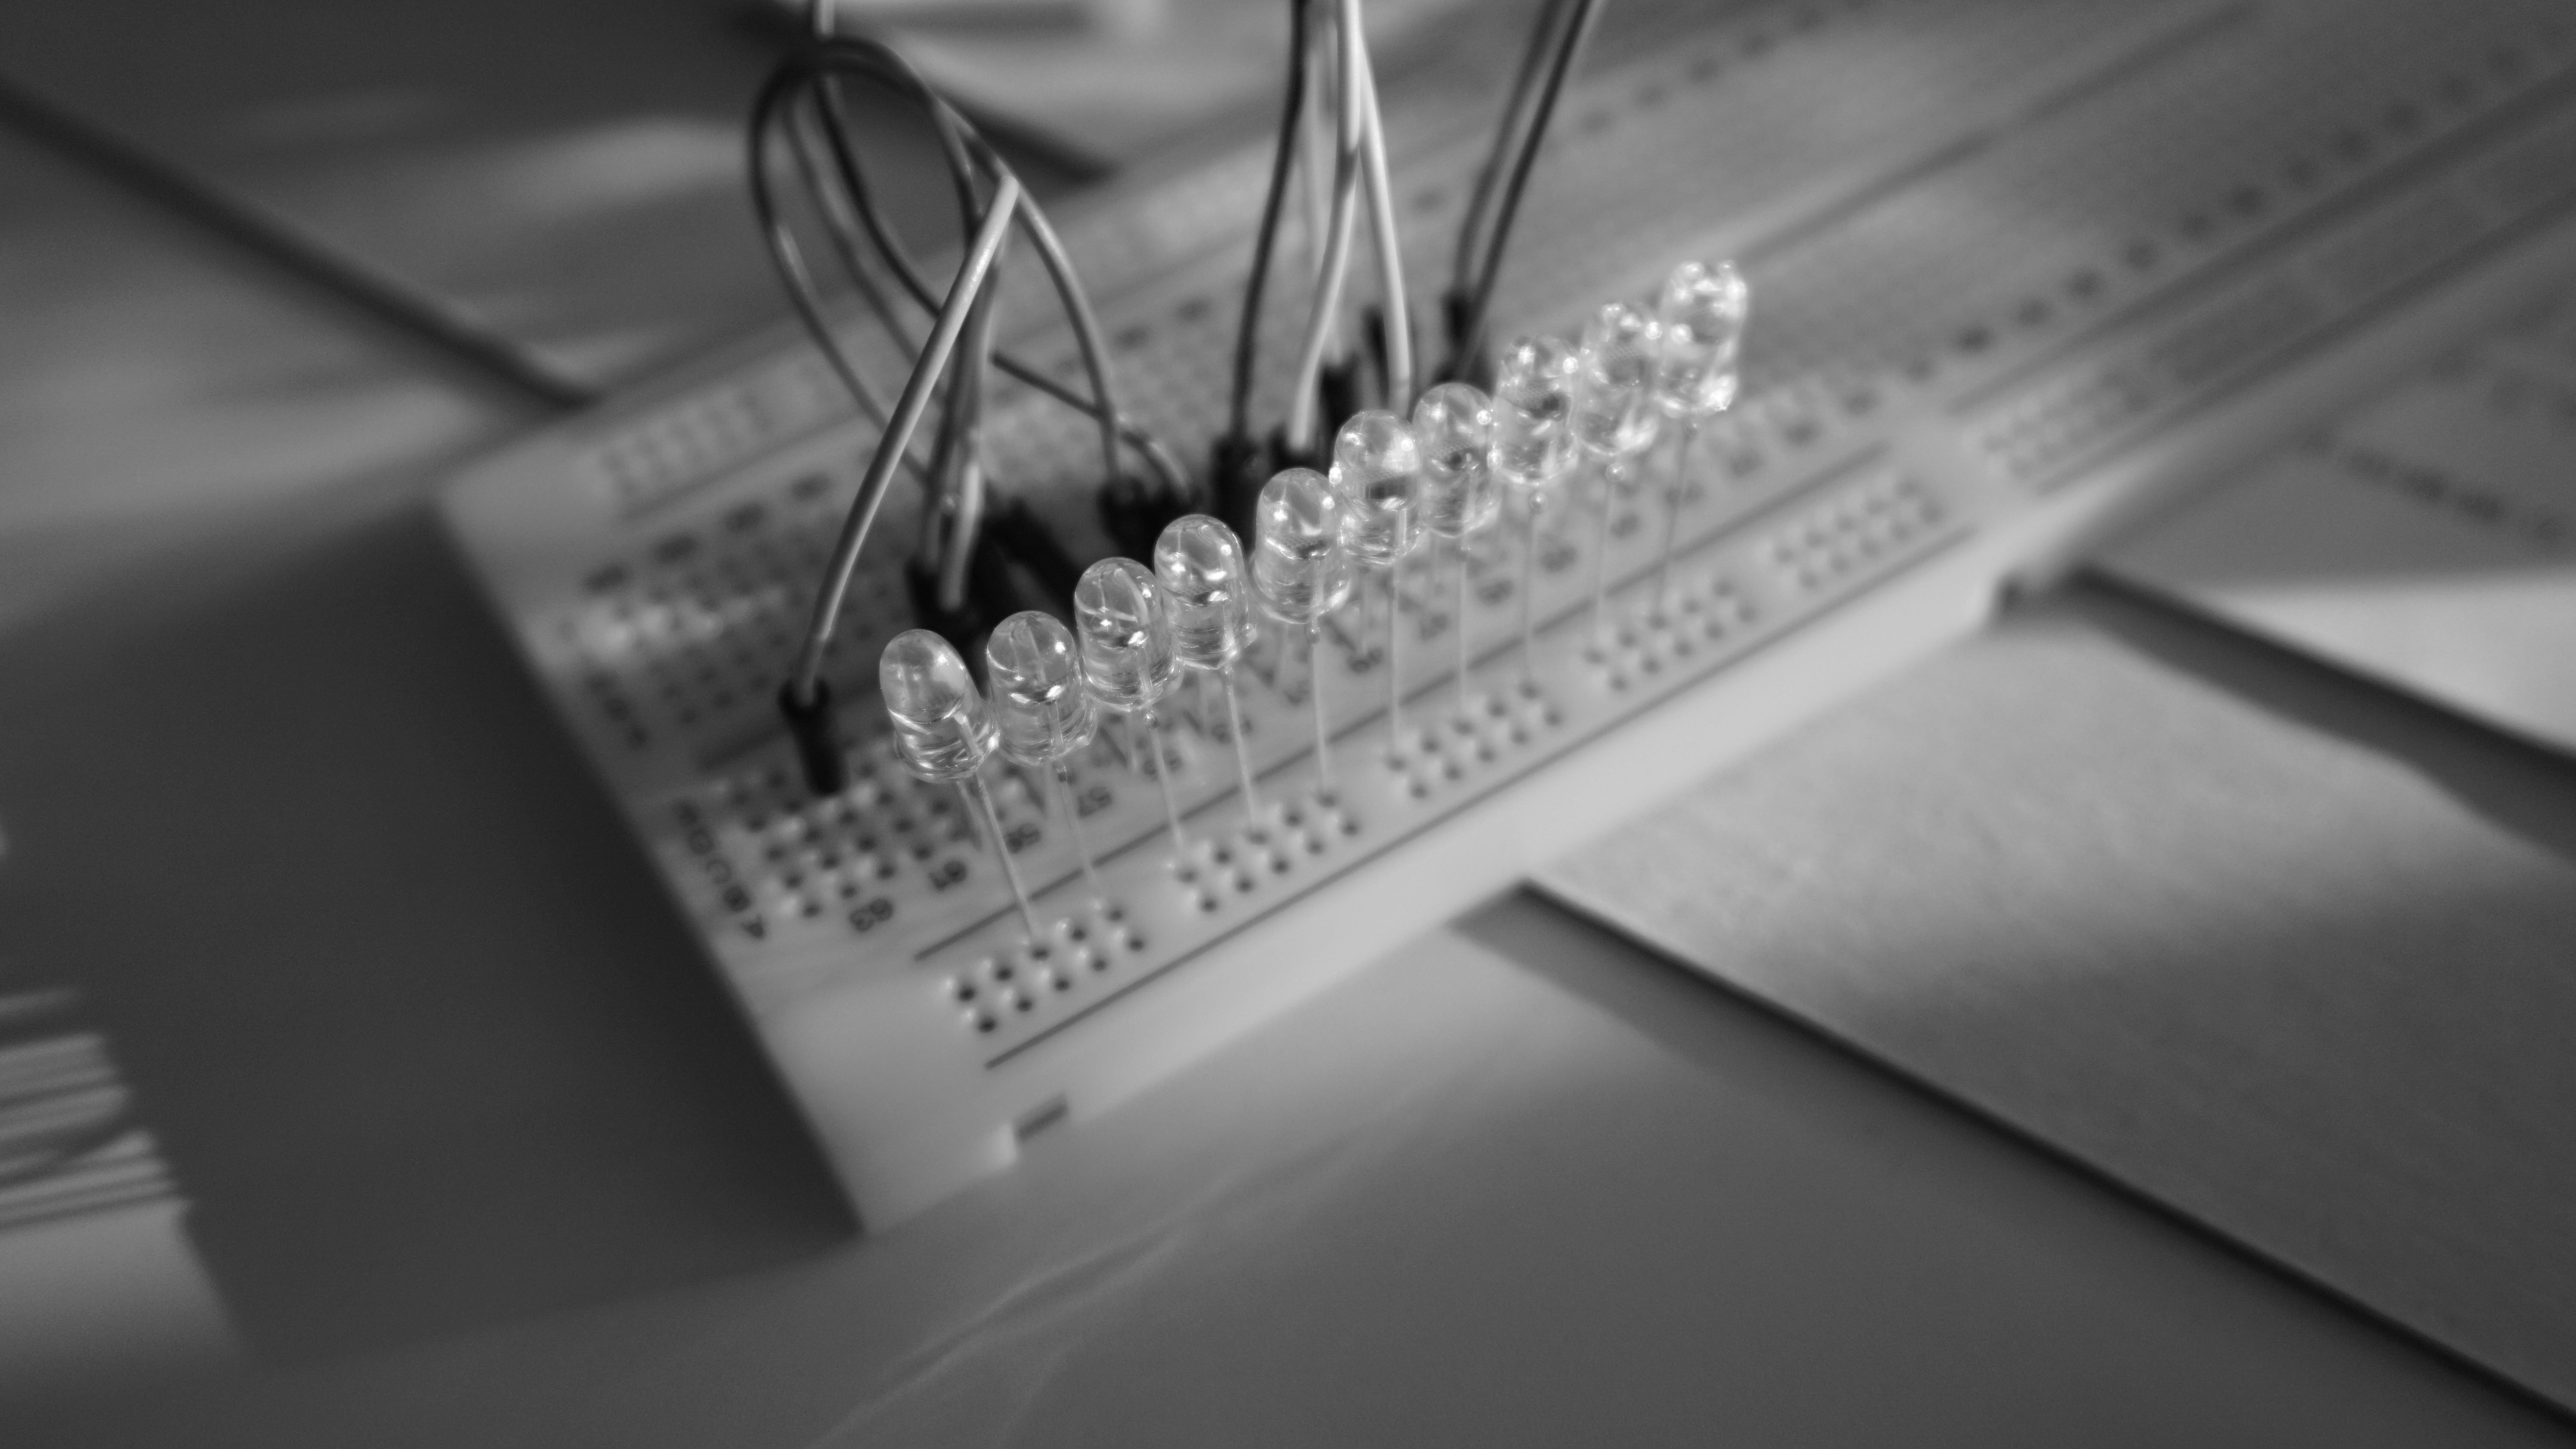
\includegraphics[width=60mm]{./assets/mouse/gray/5.JPG}
    \caption{LED10個を並列接続しているブレッドボード}
    \label{fig:led_par10}
\end{figure}

直流と並列だと並列のほうが優秀だった
並列がなんでこうなったのかはよくわからないです。
これも後ほど検証していきたいと思います。

\subsection{LEDを30個並べる}

先ほど取れたデータからだと、
LEDを30個並列に並べると1.2\si{\milli\ampere}発生するはずです。
他の実験と同じ日に行いたかったのですが、太陽が沈んでしまったので別の日に実験しました。

\begin{description}
  \item[場所]{ちかくの駐車場}
  \item[時刻]{14:30}
  \item[光源]{太陽光}
  \item[照度]{はかりわすれた}
\end{description}


\begin{figure}[htbp]
    \centering
    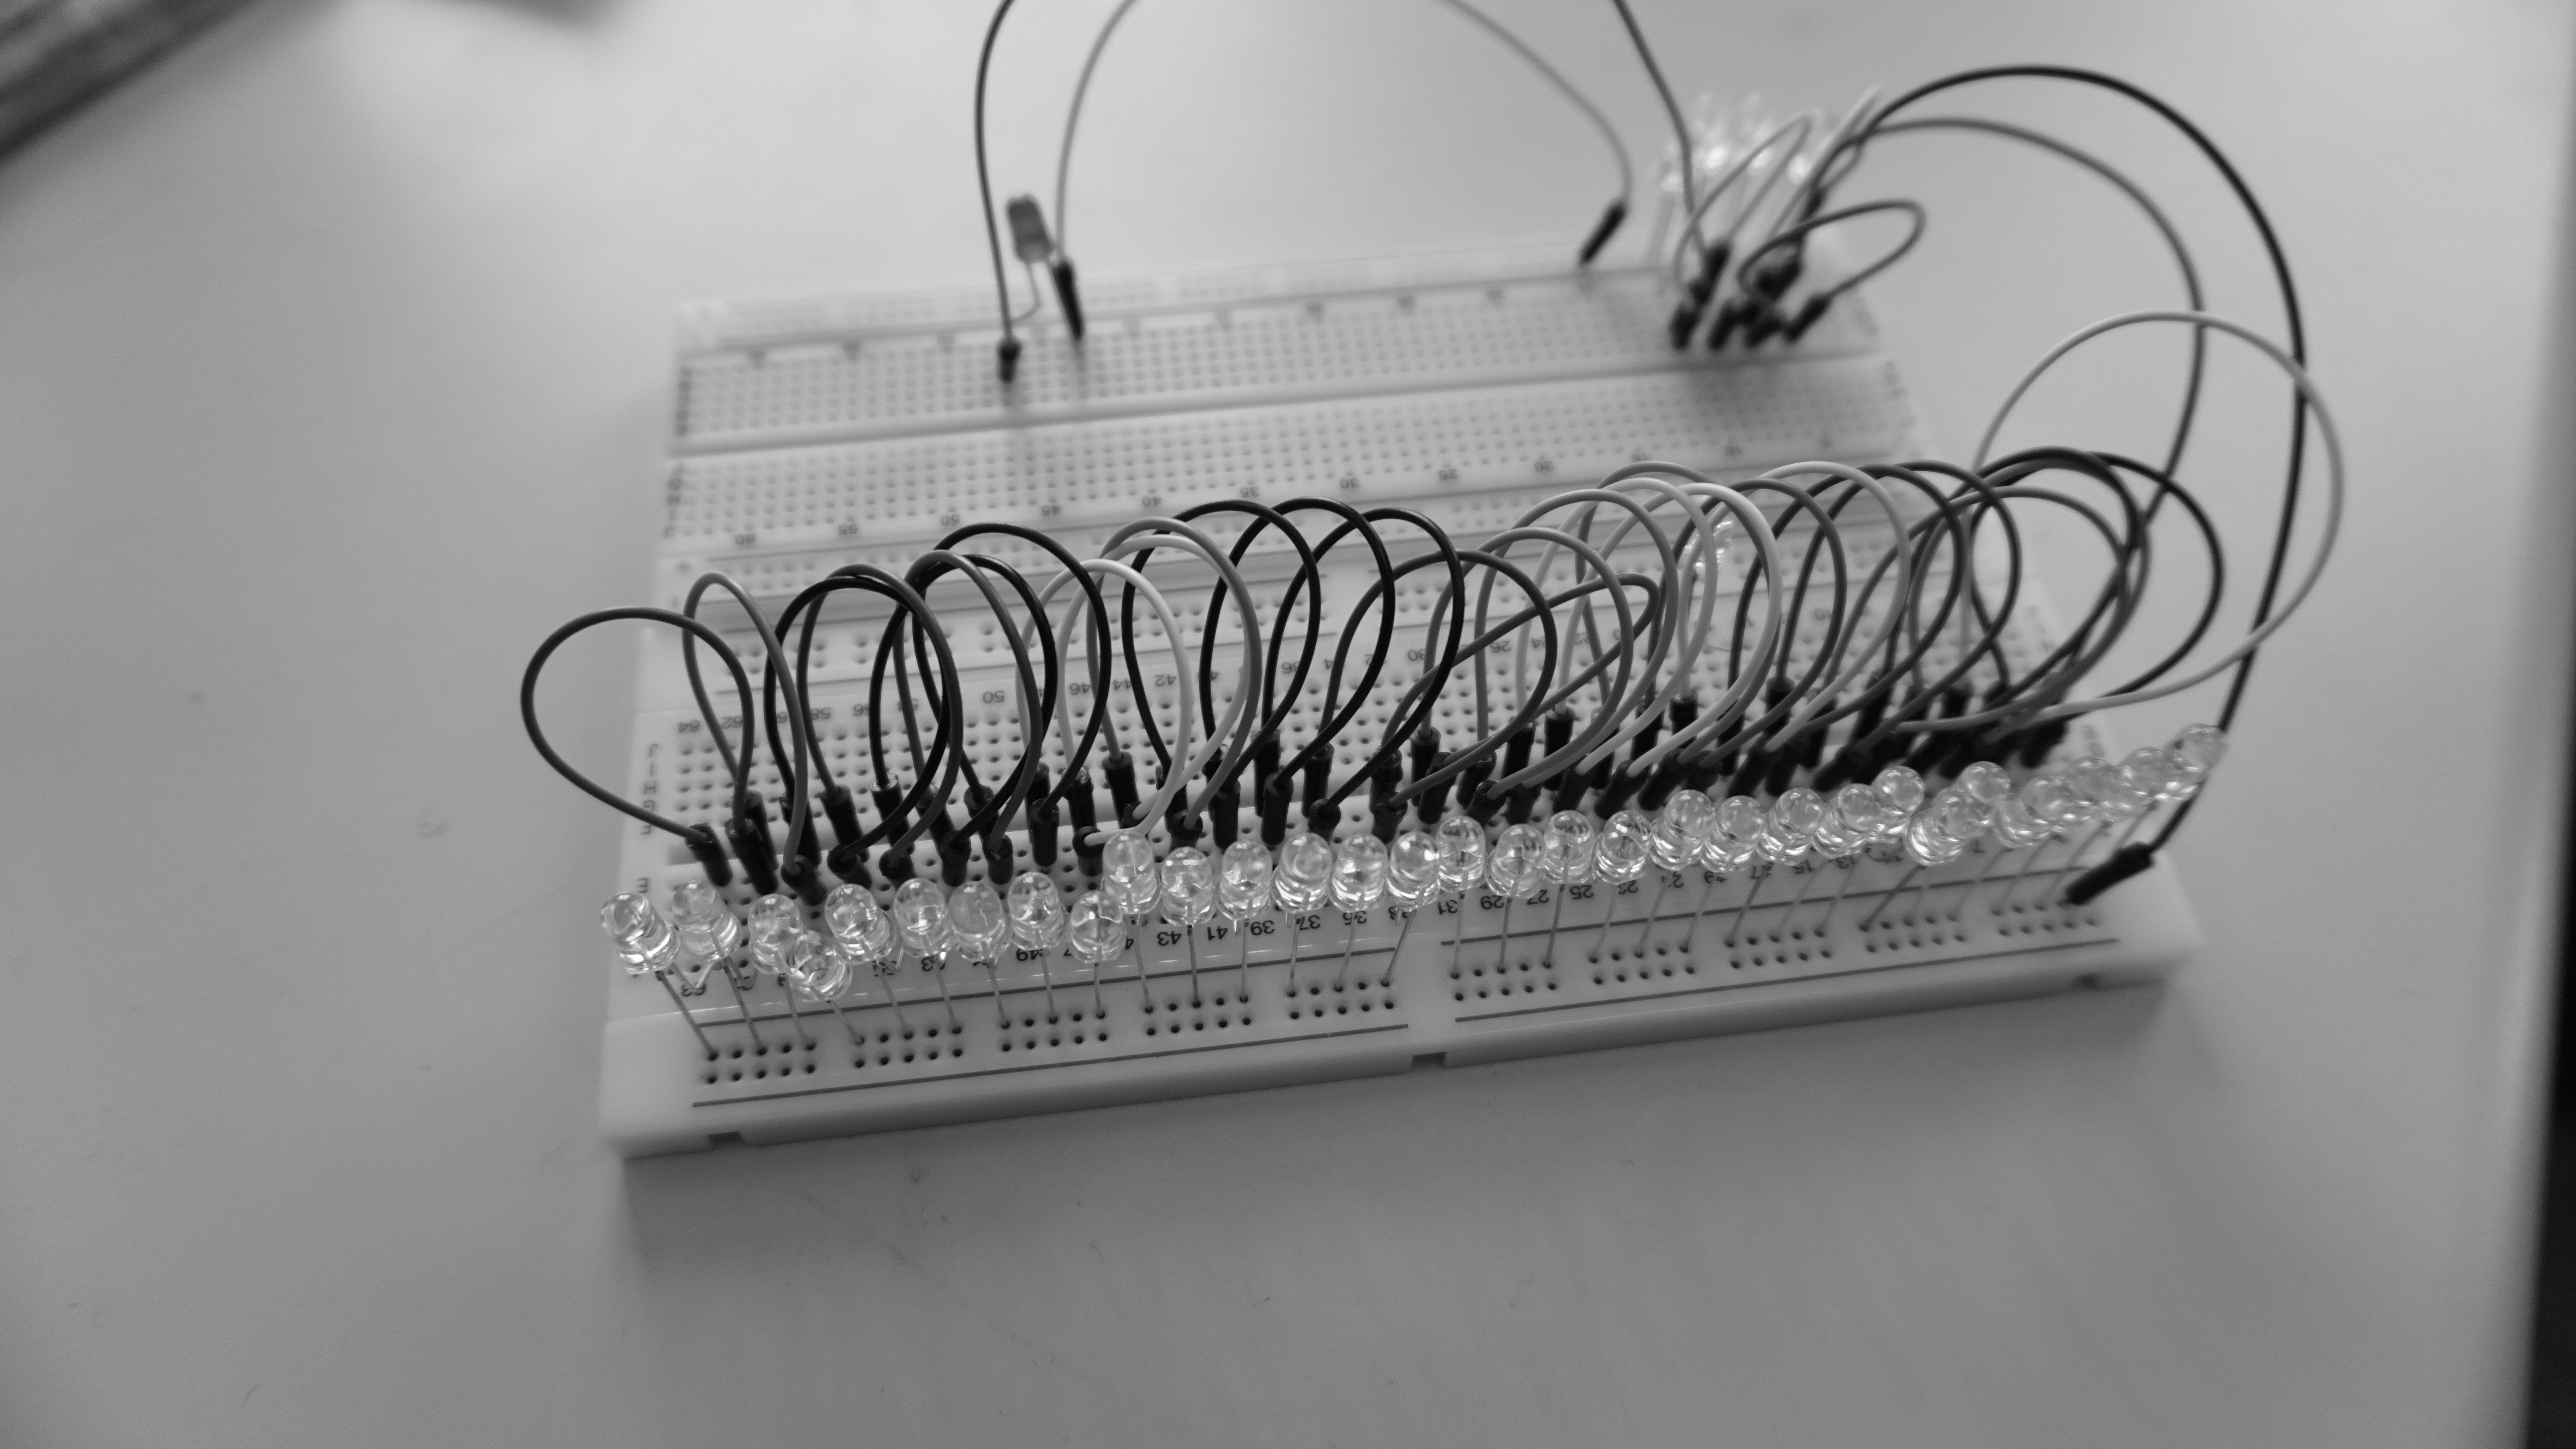
\includegraphics[width=60mm]{./assets/mouse/gray/10.JPG}
    \caption{LEDを30個並べた様子}
    \label{fig:led_par30}
\end{figure}

\newpage
図\ref{fig:led_par30}のブレッドボードを駐車場へ持って行き太陽の方へLEDを向けました。
このときは、約1\si{\milli\ampere},1.5$\si\volt$となりました。
1\si{\milli\ampere}とはさわると少しぴりぴりするかしないか程度です。また、漏電も1\si{\milli\ampere}以下が許容範囲です。つまり30個並列に並べて発生した電流は漏電にもならないのです。
悲しいですね。


\subsection{波長特性}
LEDにも波長特性はあります。
なので、LEDの色によって発電量も変わってきますし、光源の波長特性によっても全然違います。
場所、光源、LEDをしっかり選ぶとより良い発電ができるかもしれません。
今度検証してみます。

\section{最後に}
LEDで発電するのはあまりお勧めできません。
まともに使おうとしたらたくさん並べなければいけないので、とてもめんどくさいです。
だけど僕はLEDで発電することに意味があると考えているので、これからもLEDで発電していこうとおもいます。
